% $ based on Id: sample_english-v1.2.tex,v 1.2 2007/04/12 21:05:22 zlb Exp $
% $Id: sample_english.tex 6 2011-01-24 13:13:33Z hsqi $

\documentclass[english]{cccconf}
%\documentclass[usemulticol,english]{cccconf}
\usepackage[comma,numbers,square,sort&compress]{natbib}
\usepackage{amsmath}

\begin{document}

\title{LPV Multi-objective Robust Control of \\ Wind Energy Conversion System}
\author{WU Dinghui\aref{hit},
        LI Yiyang\aref{hit},
        WANG Li\aref{hit},
        JI Zhicheng\aref{hit}}

\affiliation[hit]{Institute of Electrical Automation, Jiangnan University,
					Wuxi, Jiangsu, 214112, P.~R.~China
        \email{lyyyuna@gmail.com}}

\maketitle

%--------------Abstract---------------%
\begin{abstract}
In light of the multi-time scale characteristic of the wind velocity,
and the normalized double-frequency model of wind energy conversion system
(WECS), a linear parameter varying (LPV)
model is established. The PI controller is used in the
low-frequency loop, and the $H_\infty$ gain scheduling control
method is
adopted in the high-frequency loop. Simulation results depict that
the coalition of double-frequency control compensate the controller
dynamically, and the proposed method can not only reduce the sensitivity
of system steady-state operation point, but also have better dynamic and
static characteristics.
\end{abstract}
%--------------Abstract---------------%


\keywords{Wind Energy Conversion System, LPV Model, PI Control,
Gain Scheduling Control}

\footnotetext{This work is supported by National Natural Science
Foundation (NNSF) of China(60774030); Prospective Joint Research
Project of Industry, Education and Academy of Jiangsu Province(BY2012071)}

%--------------Introduction---------------%
\section{Introduction}

For WECS, the ob1jectives of harvesting the maximum power, improving the
power quality and raising the system reliability conflict with each
other. If only one of the objectives is optimized, others are bound to
be interfered. So, it is quite necessary to choose a compromising control
method. In \cite{lit:1,lit:2}, this is realized by using linear
quadratic optimal method with the weighting coefficient chosen reasonably.
In \cite{lit:3,lit:4}, the energy conversion efficiency and
realiability are taken as the optimization objectives to design the PI controller
and linear quadratic gaussian (LQG) optimal controller. In \cite{lit:5}, it introduces
a single neuron controller to replace the active stator power PI regulator,
and the new controller is able to decouple the control of active and reactive
power, which realize the multi-objective. These control methods have overcome
the time-varying and nonlinear factors of wind turbines, which obtain
certain effects. But the wind turbine is a complex multi-variable nonlinear
system, the dynamic characteristic and system parameters are affected by
many factors in the whole operating range, like the uncertainty and measurement
error of wind velocity.

An efficient way of designing parameter dependent controller is within the
framework of LPV control. Here, a controller is synthesized to satisfy a
performance specification for all possible parameter values within a specified
model and specified rate of parameter variation. The controller can be
synthesized after solving an convex optimization problem subject to linear
matrix inequalities (LMIs).

This paper is organized as follows: Section 2 gives the WECS mechanical
model, and the normalized error LPV model is established on the basis of
\cite{lit:5,lit:6}. In Section 3, the optimization problem is presented and
the LPV controller is synthesized by $ Lyapunov $ function and LMIs with
rational weighting function. Section 4 contains a simulation result and followed
by the conclusion in Section 5.
%--------------Introduction---------------%

%--------------Model---------------%
\section{Multi-variable Model of WECS}

Based on the variable-speed variable-pitch control of WECS, and the multi-scale
characteristic of wind velocity, the normalized double-frequency model is built~\cite{lit:6,lit:7}.
The low-frequency model and the high-frequency one are given as:
\begin{equation}\label{e:1}
\begin{cases}
\overline{\Gamma_{wt}}       & = 0.5\pi\rho{}R^3\overline{v}C_\Gamma(\overline{\lambda}, \overline{\beta}) \\
J_l\dot{\overline{\Omega_l}} & = \overline{\Gamma_{wt}}-\dfrac{i}{\eta}\overline{\Gamma_G} \\
\dot{\overline{\beta}}       & = \dfrac{1}{T_\beta}(\overline{\beta_{ref}} - \overline{\beta})
\end{cases}
\end{equation}
\begin{equation}\label{e:2}
\begin{cases}
\dot{\overline{\Delta\Omega_l}}(t) & = \dfrac{1}{J_T}(\overline{\Delta\Gamma_{wt}}(t) - \overline{\Delta\Gamma_G}(t)) \\
\dot{\overline{\Delta\beta}} & = \dfrac{1}{T_\beta}(\overline{\Delta\beta_{ref}} - \overline{\Delta\beta}) \\
\dot{\overline{\Delta\Gamma_{wt}}}(t) & = (\dfrac{\gamma}{J_T} - \dfrac{1}{T_w} )\overline{\Delta \Gamma_{wt} }(t) \\
				& + \dfrac{\gamma }{T_w}\overline{\Delta \Omega_l }(t) + (\dfrac{\zeta }{T_w} - \dfrac{\zeta }{T_\beta })
				\overline{\Delta\beta}(t) \\
				& - \dfrac{\gamma}{J_T}\overline{\Delta\Gamma_G}(t) + \dfrac{\zeta }{T_\beta}\overline{\Delta \beta_{ref}}(t)
				+ \dfrac{2-\zeta}{T_w}e(t) \\
\end{cases}
\end{equation}
where $T_{wt}$ is the wind torque produced by the wind turbine, $C_p$ is the wind
energy conversion coefficient, $C_\Gamma$ is the wind torque coefficient, $\lambda $
is the tip speed ratio, $\beta$ is the pitch angle, $R$ is the rotor radius of the
wind turbine, $\eta$ is the air density, $\Omega_l$ is the rotor speed, $v$ is the
wind velocity, $i$ is the gear ratio, $\Gamma_G$ is the electromagnetic torque,
$\eta$ is the gear efficiency and $J_T$ is the inertia.

In order to describe the WECS operation status accurately,
$\rho(t)=[\gamma(t), \zeta(t)]^T$ is taken as the time-varying parameter. Inside the
double-frequency loop, the parameter $J_T, T_w$ vary far more slowly than $\gamma, \zeta$,
so $J_T$ and $T_w$ can be valued as constant. From Eq.\ref{e:1} and Eq.\ref{e:2}, the
linear time-varying state equation is given as:
\begin{equation}\label{e:3}
\dot{x}(t)=A(\rho(t))x(t) + B(\rho(t))u(t) + L(\rho(t))e(t)
\end{equation}
where the state vector $x(t)$ is $[\overline{\Delta\Omega_l}(t), \overline{\Delta\beta}(t),
\overline{\Delta\Gamma_{wt}}(t)]^T$, and the control input vector $u(t)$ is
$[\overline{\Delta\Gamma_G}(t), \overline{\Delta\beta_{ref}}(t)]^T $. The coefficient matrix
$L(\rho(t))$ is $[0, 0, (2-\gamma(t))/T_w]^T$, $A(\rho(t))$ is
$ \begin{bmatrix}
0 & 0 & \dfrac{1}{J_T} \\
0 & -\dfrac{1}{T_\beta} & 0 \\
\dfrac{\gamma(t)}{T_w} & \dfrac{\zeta(t)}{T_w}-\dfrac{\zeta(t)}{T_\beta} & \dfrac{\gamma(t)}{J_T}-\dfrac{1}{T_w}
\end{bmatrix}
$, \newline
$B(\rho(t))$ is
$\begin{bmatrix}
-\dfrac{1}{J_T} & 0 \\
0 & \dfrac{1}{T_\beta} \\
-\dfrac{\gamma(t)}{J_T} & \dfrac{\zeta}{T_\beta}
\end{bmatrix}$.

The objective of WECS can be divided into two parts: When the wind velocity is below the
rated one, the objective is to reduce the error of  tracking the optimal value $lambda_{opt}$
from the high-frequency component. While the velocity is above the rated one, the
objective is to keep the generated power and rotor speed at the rated value. Meanwhile,
the amplitude and frequency of the electromagnetic torque oscillation should be taken
into consideration. From the above, the system output vector is defined as:
\begin{equation}\label{e:4}
z(t)=\begin{bmatrix}
\overline{\Delta\lambda}(t) \\
\overline{\Delta{}P_e}(t) \\
\overline{\Delta\Omega_h}(t) \\
\end{bmatrix}
=C(\rho(t))x(t) + Du(t)
\end{equation}
where, $\overline{\Delta\lambda}(t) = \overline{\Delta\Omega_l}(t) -
\dfrac{1}{2-\gamma}\overline{\Delta\Gamma_{wt}}(t) + \dfrac{\gamma}{2-\gamma}\overline{\Delta\Omega_l}(t)$,
$P_e$ is the power of generator,  and $P_e = \Omega_h\Gamma_G$,
$\overline{\Delta{}P_e}(t) = \overline{\Delta\Omega_h}(t) + \overline{\Delta\Gamma_G}(t)$,
$\overline{\Delta\Omega_h}(t) = \overline{\Delta\Omega_l}(t)$.
Then the coefficient matrix in Eq.\ref{e:4} can be deduced as:
$C(\rho(t)) = \begin{bmatrix}
2/(2-\gamma(t) & 0 & 1/(2-\gamma(t)) \\
1 & 0 & 0 \\
1 & 0 & 0
\end{bmatrix}$,
$D = \begin{bmatrix}
0 & 0 \\
1 & 0 \\
0 & 0
\end{bmatrix}$.

The Eq.\ref{e:3} and Eq.\ref{e:4} constitute the normalized error LPV model of WECS,
and the coefficient matrix is affine dependent on the parameter vector $\rho(t)$.
%--------------Model---------------%

%--------------Control---------------%
\section{Multi-variable Control of WECS}

This section presents LMIs based method for designing and synthesizing of the 
double-frequency loop gain scheduling controller of WECS. The  low-frequency 
loop adopts PI control while the high-frequency loop uses
LPV control method as a dynamic compensation which is based on the normalize error.

%%%%%%%%%%%%%%%%%%%%%%%%%%%%%%%%%%%%%%
%--------subsection------------------%
\subsection{PI Optimization of the Low-frequency Loop}

Different objective is selected under different wind velocity:
When the wind velocity is under the rated one, the pitch is kept at the
optimal value. To capture the maximum power, the low-frequency component
of rotor speed $\overline{\Omega_l}$ is controlled to track the reference
$\overline{\Omega_{ref}}=\lambda_{opt}\overline{v}/R$ using the PI method.
When the wind velocity is above the rated one, the pitch angle $\beta$ and
generator torque $\Gamma_G$ are controlled together to keep the power at
a constant.

(1) power control:

The power error is defined as: $\Delta{}P=P_{ref}-P$.

The first-order dynamic process of power error is:
\begin{equation}\label{e:5}
  \Delta\dot{P}+c_0\Delta{}P=0, c_0>0
\end{equation}

Take $P_e=\Omega_h\Gamma_G$ into account, the following can be obtained
from Eq.\ref{e:5}:
\begin{equation}\label{e:6}
  -\dot{\Omega_h}\Gamma_G-\Omega_h\dot{\Gamma_G}+c_0\varepsilon_p=0
\end{equation}

Then the torque reference can solved out from Eq.\ref{e:5} and
Eq.\ref{e:6}:
\begin{equation}\label{e:7}
  \dot{\Gamma}_{ref}(t) = \dfrac{1}{\Omega_h(t)}[c_0\varepsilon_p(t) -
        \dfrac{1}{J_h}(\dfrac{\eta}{i}\Gamma_{wt}(t)\Gamma_G(t)-\Gamma^2_G(t))]
\end{equation}

(2) rotor speed control

The pitch reference can be calculated from the following:
\begin{equation}\label{e:8}
  \beta_{ref}(t) = K_{P2}\Delta(t) + K_{I2}\int\Delta\Omega(t)
\end{equation}
where the rotor speed error is $\Delta\Omega(t)=\Omega_{ref}-\Omega_h(t)$,
and the propotional and integral coefficient is $K_{P2}, K_{I2}$.


%%%%%%%%%%%%%%%%%%%%%%%%%%%%%%%%%%%%%%
%--------subsection------------------%
\subsection{LPV Control of High-frequency Loop}

For the high inertia of the wind turbine and the randomness of the wind
velocity, the PI control of the low-frequency loop will produce large
torque variation on the shaft of the motor. As a result of the limitation
of the response speed of the pitch servo motor and generator, the whole
mechanical subsystem will become unreliable. To make up this shortcoming,
the LPV gain scheduling control is introduced to optimize
the high-frequency component dynamically. As the LPV focuses more on the
variation of the operation point by adjusting the controller's parameter
real-time, the sensitivity of the steady state can be reduced remarkably.

From Eq.\ref{e:3}, there exist external interference and error of the linear
model. To restrain the compact of the wind velocity and the model error, the
$H_\infty$ controller $K(s)$ is designed, which is based on the LPV model.
The controller is to make the $H_\infty$ norm of the closed-loop transfer
function $T_{ez}(s)$ from the external interference $e(t)$ to the control
input $z(t)$ less than a given performance objective $\gamma$:
\begin{equation}\label{e:9}
  \| T_{ez}(s) \|_\infty < \gamma
\end{equation}

Assuming that the open-loop LPV system from Eq.\ref{e:3} is dependent on
the trajectory of the parameter $\rho(t)$, there exists two independent
symmetric matrix parameters $X, Y$, as well as four independent matrix
parameters $\hat{A}, \hat{B}, \hat{C}, \hat{D}$, which will make all $\rho$
satisfy
\begin{equation}\label{e:10}
  \begin{bmatrix}
  \begin{smallmatrix}
    \dot{X}+XA+\hat{B}C_2   &   \ast    &   \ast    &   \ast    \\
    \hat{A^T}+A+B_2\hat{D}C_2   & -\dot{Y}+AY+B_2\hat{C}+{\ast} & \ast & \ast \\
    (XB_1+\hat{B}D_{21})^T  & (B_1+B_2\hat{D}D_{21})^T & -\gamma{I_{n_w}} & \ast \\
    C_1+D_{12}D\hat{C}_2 & C_1{}Y+D_{12}\hat{C} & D_{11}+D_{12}\hat{D}D_{21} & -\gamma{}I_{n_z}
  \end{smallmatrix}
  \end{bmatrix}
  <0
\end{equation}
\begin{equation}
    \begin{bmatrix}\label{e:11}
  X &   I   \\
  I &   Y
  \end{bmatrix}>0
\end{equation}
then there exists a controller\cite{lit:8,lit:9}, such that\newline
(1) The closed-loop is parameter dependent quadratic (PDQ) stable in the varying
    range of $\theta(t)$. \newline
(2) The induced $L_2{}-norm$ of the operator $T_{zw}$ is bounded by $\gamma>0$
    (i.e. $\| T_{zw}\|_{i,2} < \gamma $ ).


The next step is to find a appropriate LPV controller:
\begin{equation}\label{e:12}
  \begin{cases}
    \dot{x_c}(t) & = A_c(\rho(t))x_c(t) + B_c(\rho(t))y(t) \\
    u(t) & = C_c(\rho(t))x_c(t) + D_c(\rho(t))y(t)
  \end{cases}
\end{equation}
and the four control matrixes are shown below
\begin{equation*}
  \begin{split}
    A_c(\rho) & = N^{-1}(\rho)(N(\rho)M^T(\rho) + \hat{A}(\rho) - \hat{B}(\rho)C_2(\rho)Y \\
              & X(A(\rho) - B_2(\rho)\hat{D}(\rho)C_2(\rho)Y - XB_2(\rho)\hat{C}(\rho)M^{-T}(\rho)) \\
    B_c(\rho) & = N^{-1}(\rho)(\hat{B}(\rho) - XB_2(\rho)\hat{C}(\rho)) \\
    C_c(\rho) & = (\hat{C}(\rho) - \hat{D}(\rho)C_2(\rho)Y)M^{-T}(\rho) \\
    D_c(\rho) & = \hat{D}(\rho)
  \end{split}
\end{equation*}

Then the high-frequency loop controller is simplified as a mixed sensitivity
problem, as illustrated in Fig.\ref{fig1}
\begin{figure}[!htb]
  \centering
  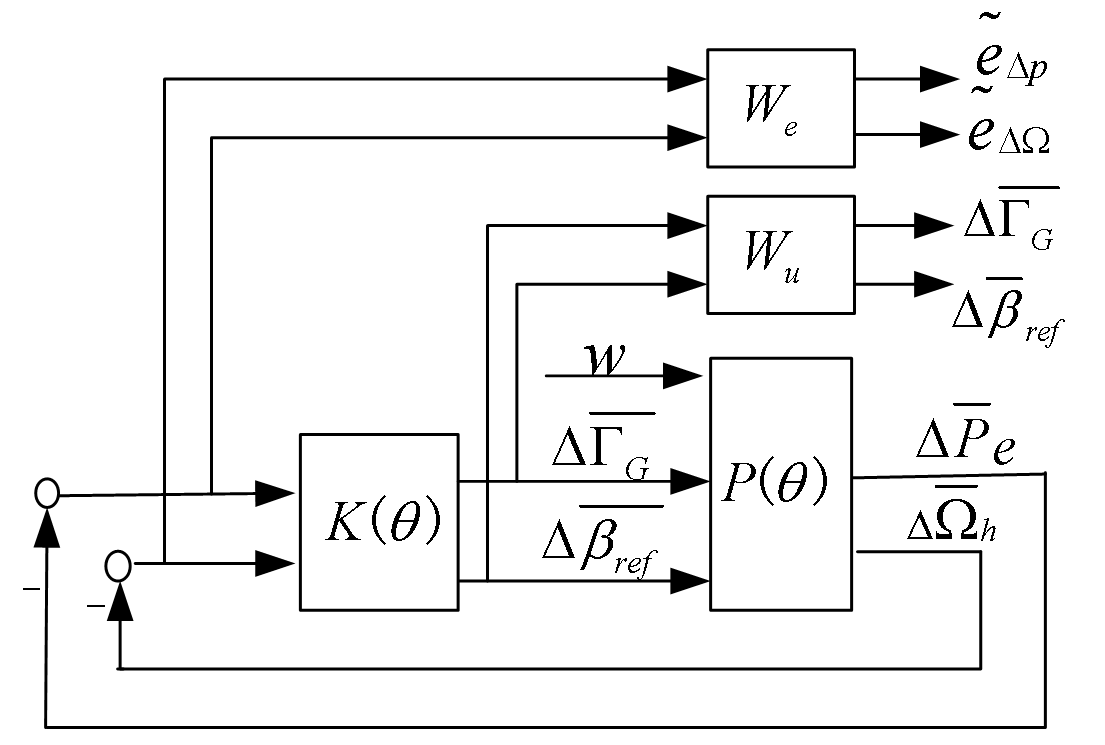
\includegraphics[width=\hsize]{1.png}
  \caption{$H_\infty$ Control with Multi-variable controllers}
  \label{fig1}
\end{figure}

In the figure, $\Delta\overline{P}_e, \Delta\overline{\Omega}_l$ are the
controlled variables, $\overline{\Delta\Gamma_G}(t), \overline\beta_{ref}(t)$
are the control signals and $w$ is the wind interference. When the rotational
speed is at different operating range, the objective is different. In the
synthesis model from Fig.\ref{fig1}, the excepted output performance can be
obtained by designing the appropriate sensitivity weighting function $W_e(s)$
and control weighting function $W_u(s)$.

The $W_e(s)$ emphasizes the importance of error component, and improves the
tracking performance and the restraint of external disturbance. While the
$W_u(s)$ weights the control effects, which guarantee the output limitation
to meet the real application restriction. The selection of the weighting
function directly reflects the requirement of the system performance
in the $H_\infty$ optimization, so it is necessary to choose the
low-order weighting function as far as possible.

Sensitivity weighting function $W_e(s)$ can restrain the disturbance of
the wind velocity and can accurately track the speed and power
reference according to \cite{lit:10}.
The high-frequency wind velocity spectrum is $0.06 - 0.7m/s$ which is
quite considerable, so when the wind velocity is below the rated one,
$[k_{wel1}, k_{wel2}]$ is $[1, 10]$, and when above the rated one,
$[k_{weh1}, k_{weh2}]$ is $[0.05, 0.01]$. The control variable must be
limited by the weighting function $W_u(s)$.
If the torque and pitch
frequency is too high, and the variation scope is too large, it will
bring mechanical vibration and impact on the reliability of the general
system. According to the actual situation, when the wind velocity is
below the rated one, $[k_{wul1}, k_{wul2}]$ is $[1, 10]$, and when above
rated one, $[k_{wuh1}, k_{wuh2}]$ is $[0.01, 0.3]$. In the whole control
process, $k_{e1}, k_{e2}, k_{u1}, k_{u2}$ in the weighting function
is affine dependent on $\rho$
\begin{equation}\label{e:13}
  \begin{cases}
    k_{e1}(\rho) & = \phi_e(\rho)k_{wel1} + (1 - \phi_e(\rho))k_{weh1}  \\
    k_{e2}(\rho) & = \phi_e(\rho)k_{wel2} + (1 - \phi_e(\rho))k_{weh2}  \\
    k_{u1}(\rho) & = \phi_u(\rho)k_{wul1} + (1 - \phi_u(\rho))k_{weu1}  \\
    k_{u2}(\rho) & = \phi_u(\rho)k_{wul2} + (1 - \phi_u(\rho))k_{weu2}
  \end{cases}
\end{equation}

And the final weighting function is shown below.
\begin{equation}\label{e:14}
  W_e(s) = \begin{bmatrix}
            k_{e1} & 0 \\
            0 & k_{e2}
            \end{bmatrix}
            \dfrac{s/100+1}{s}
\end{equation}
\begin{equation}\label{e:15}
  W_u(s) = \begin{bmatrix}
    k_{u1}\dfrac{s/(0.1\omega_1)+1}{s/(10\omega_2)+1}   &  0 \\
    0   &   k_{u2}\dfrac{s/(0.1\omega_2)+1}{s/(10\omega_2)+1}
  \end{bmatrix}
\end{equation}
%--------------Control---------------%


%--------------Simulation---------------%
\section{Simulation}

The multi-variable controller output is the steady-state component of the
total control input of the WECS. The LPV dynamic compensation controller's
output is the dynamic part of the normalized one. So the output is described
in Eq.\ref{e:16} and Eq.\ref{e:17}. Where $\overline{\Gamma_{Gref}}(t),
\overline{\beta_{Gref}}(t)$ are the multi-variable control input,
$\overline{\Delta\Gamma_{Gref}}(t), \overline{\Delta\beta_{Gref}}(t)$ are
the LPV dynamic compensation control output. The compensation intensity
of LPV control is described by the coefficient $k_{\Gamma}$ and $k_\beta$.
\begin{equation}\label{e:16}
  \Gamma_{Gref}(t)  = \overline{\Gamma_{Gref}}(t) +
                    k_\Gamma\dfrac{\overline{\Delta\Gamma_{Gref}}(t)}
                    {\overline{\Gamma_{Gref}}(t)}
\end{equation}
\begin{equation}\label{e:17}
  \beta_{Gref}(t)  = \overline{\beta_{Gref}}(t) + k_\beta\dfrac
        {\overline{\Delta\beta_{Gref}}(t)}{\overline{\beta_{Gref}}(t)}
\end{equation}

The variation spectrum of the parameter $\rho$ is evenly divided by the
grid method and value of $[\gamma(t), \zeta(t)]^T$ is observed online.
The Stability condition Eq.\ref{e:11} and Eq.\ref{e:12} form a group of
LMIs, and with the help of the LMI toolbox in $Matlab$, a feasible solution
can be figured out. The simulation parameters are shown in Tab.\ref{tab1}
\begin{table}[!htb]
  \centering
  \caption{Parameters' Value}
  \label{tab1}
  \begin{tabular}{c|c}
    \hhline
    Parameter     &     Value   \\ \hline
    $R$           &     $2.5m$  \\ \hline
    $i$           &     $6.25$  \\ \hline
    $J_T$         &     $0.236kgm^2$    \\ \hline
    $L_t$         &     $150m$  \\ \hline
    $T_w$         &     $10s$   \\ \hline
    $P_{ref}$     &     $6000W$ \\ \hline
    $\Omega_{ref}$  &   $200rad/s$  \\  \hline
    $\eta$      &   0.95    \\  \hline
    $T_\beta$   &   0.05s   \\  \hline
    $\Gamma_{Gmax}$ &   40Nm    \\  \hline
    $J_g$       &   $0.01kgm^2$ \\  \hline
    $J_t$       &   $0.09kgm^2$ \\
    \hhline
  \end{tabular}
\end{table}

To see the full operation situation of WECS, simulation of duration
$300s$ is conducted both with wind velocity below the rated one for
the first $150s$ and the second $150s$ above the rated one.
The curve is depicted in Fig.\ref{fig2}
\begin{figure}[!htb]
  \centering
  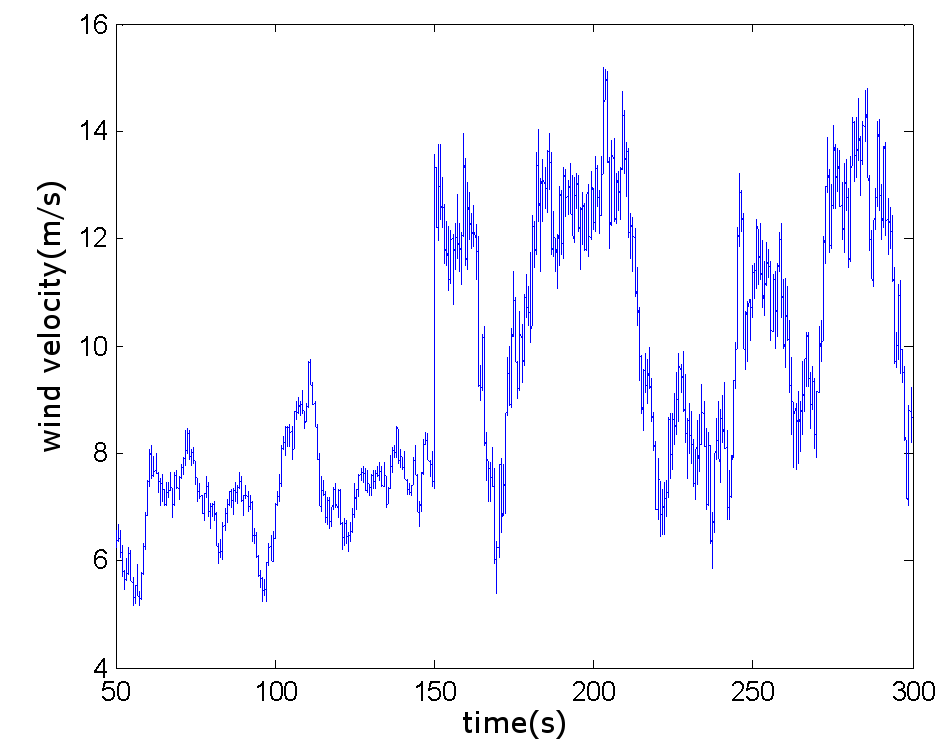
\includegraphics[width=\hsize]{2.png}
  \caption{Simulation Curve of Wind Velocity}
  \label{fig2}
\end{figure}

The wave of wind power, rotor speed, torque and pitch angle are shown
from Fig.\ref{fig3} to Fig.\ref{fig6}.
\begin{figure}[!htb]
  \centering
  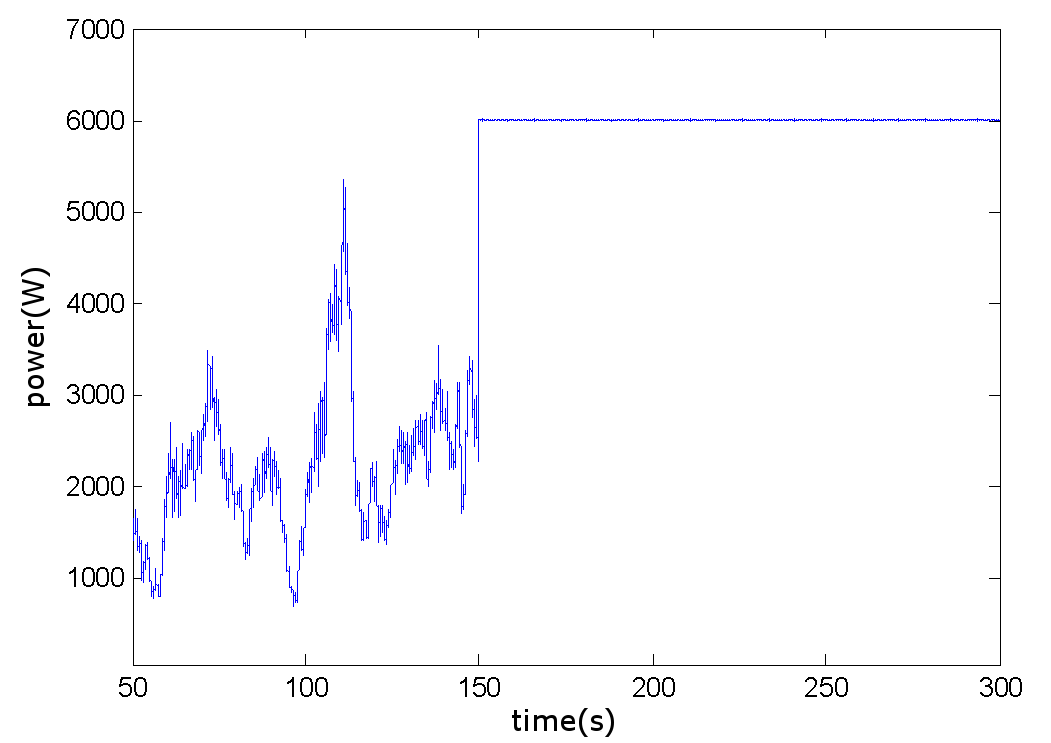
\includegraphics[width=\hsize]{3.png}
  \caption{Simulation Curve of Power Output}
  \label{fig3}
\end{figure}

\begin{figure}[!htb]
  \centering
  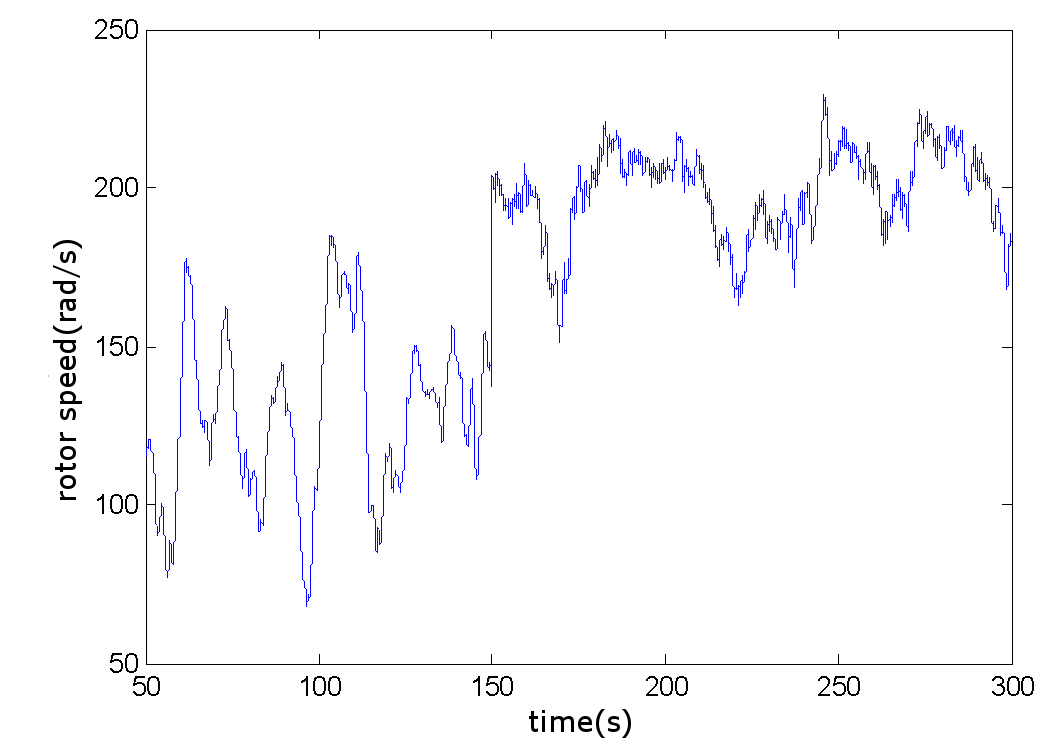
\includegraphics[width=\hsize]{4.png}
  \caption{Simulation Curve of Rotor Speed}
  \label{fig4}
\end{figure}

\begin{figure}[!htb]
  \centering
  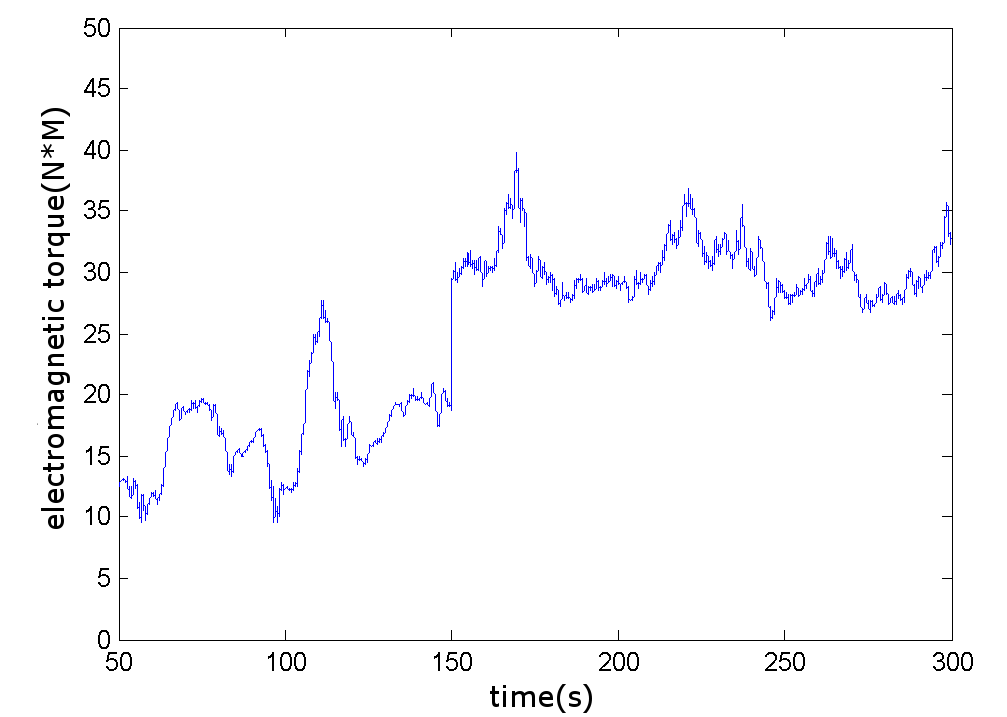
\includegraphics[width=\hsize]{5.png}
  \caption{Simulation Curve of Electromagnetic Torque}
  \label{fig5}
\end{figure}

\begin{figure}[!htb]
  \centering
  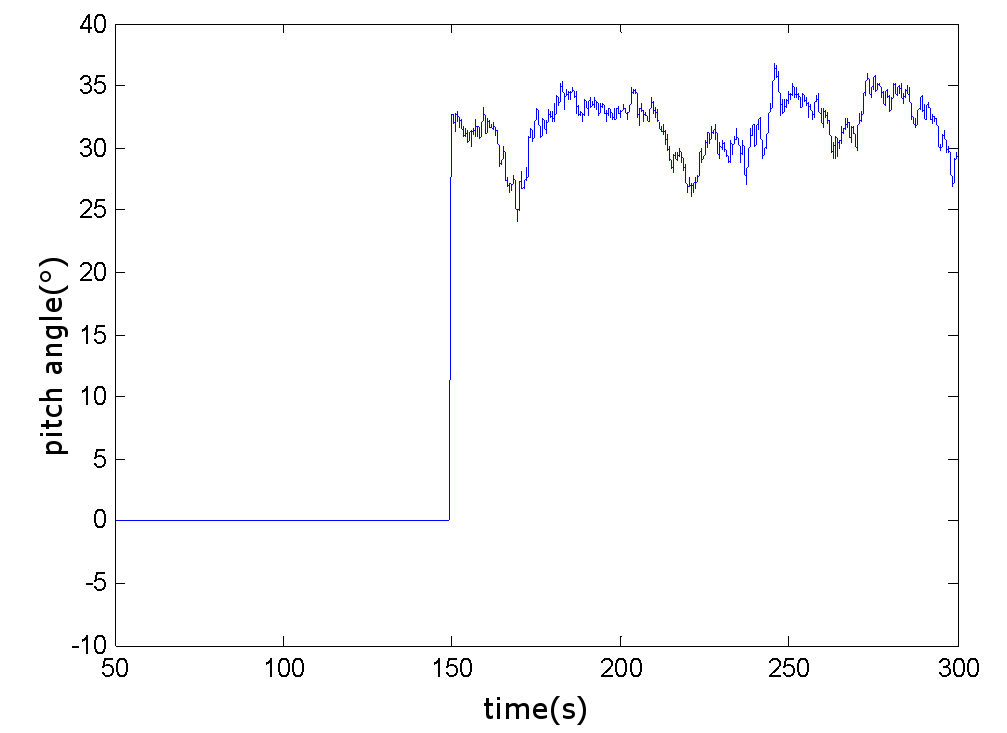
\includegraphics[width=\hsize]{6.png}
  \caption{Simulation Curve Pitch Angle}
  \label{fig6}
\end{figure}

The above figure demonstrate that when the wind velocity is below the
rated one, the pitch angle remains constant to capture the maximum energy,
and when above the rated one, the torque and pitch are controlled together
to maintain the power constant and reduce the torque oscillation. The
simulation result show that the multi-objective control based on LPV
method is efficient.
%--------------Simulation---------------%

%--------------Conclusion---------------%
\section{Conclusion}

This paper addresses the design of multi-objective controller based on LPV
method for the double-frequency model of WECS in the full operation region.
The controller handles both the parameter variations along the nominal
operating trajectory and parameter variations introduced by the wind
velocity turbulence.

Simulation show that the multi-variable controller is compensated by the
double-frequency loop method compared with the conventional one. In general,
the adopted method reduces the sensitivity of the relative steady-state
remarkably, and achieves better dynamic and static characteristics.
%--------------Conclusion---------------%

%%%%%%%%%%%%%%%%%%%%%%%%%%%%%%%%%%%%%%%%%%%%%%
%----------------bibliography----------------%
\begin{thebibliography}{0}
\bibitem{lit:1}
I.~Munteanu, A.~Bratcu, N.A.~Cutululis, A Two Loop Optimal Control of Flexible
Drive Train Variable Speed Wind Power Systems, in \emph{Proceedings of the 16th
IFAC Word Congress}, 4--8, 2005.

\bibitem{lit:2}
I.~Munteanu, N.A.~Cutululis, A.~Bratcu, Using a Nonlinear Controller to Optimize
a Variable Speed Wind Power System, \emph{Journal of Electrical Engineering},
 6(4): 147-154, 2006.

\bibitem{lit:3}
B.~Boukhezzar, L.~Lupu, H.~Siguerdidjane, M.~Hand, Multivariable Control Strategy
for Variable Speed, Variable Pitch Wind Turbine, \emph{Renewable Energy}, 32(8):
1273--1287, 2007.

\bibitem{lit:4}
M.~Steinbuch, Optimal Multivariable Control of a Wind Turbine with Variable Speed,
\emph{Wind Engineering}, 11(3): 153--163, 1987.

\bibitem{lit:5}
Yang Yong, Ruan Yi, Ren Zhibing, Single Neuron Controller of VSCF Wind Power
Generation System, \emph{Micromotors}, 42(9): 60--65, 2009.

\bibitem{lit:6}
Wu Dinghui, Ji Zhicheng, Two-Frequency-Loop Optimal Control for Wind Energy
Conversion System Based on $ H_\infty $, \emph{Journal of Jiangnan University},
6: 683--687, 2009.

\bibitem{lit:7}
Inlian Munteanu, Antoneta Iuliana Brarcu, Nicolaos Antonic Cutululis, Optimal
Control of Wind Energy Systems, Springer, 2008.

\bibitem{lit:8}
Chen Wang, George Weiss, Self-scheduled LPV Control of a Wind Driven
Doubly-Fed Induction Generator, in \emph{Proceedings of the 45th IEEE Conference on
Decision}, 1246--1251, 2006.

\bibitem{lit:9}
Deng Ying, Zhou Jie, LPV $ H_\infty $ Controller Design for a Wind Power Generator,
in \emph{2008 IEEE}, 873--878, 2008.

\bibitem{lit:10}
P.~A.~Pkarian, P.~G.~Ahinet, G.~Becker, Self-scheduled $ H_\infty $ Control of
Linear Parameter-varying Systems: a Design Example, \emph{Automatica}, 31(9),
1251--1261, 1995.

\end{thebibliography}
%----------------bibliography----------------%

\end{document}
